
%------------------------------------------------

\section{Pseudorandom numbers and Monte Carlo methods}
\label{sec:pseudorandom_number}

\subsection{Pseudorandom number generator}\index{pseudorandom number}
\label{subsec:pseudorandom_number_generator}

So far, we have used random numbers in almost all exercises, without actually explaining what they are and what are their properties and limitations. 

A pseudorandom number generator is an algorithm that generates a sequence of numbers distributed according to some PDF and that resemble very closely an actual distribution of random numbers with the same PDF.

\subsection{Properties of pseudorandom number generator}\index{pseudorandom number!property}
\label{subsec:prop_of_pseudorandom_number_generator}

\begin{itemize}[$\to$]
	\item Each extraction must be statistically independent from previous ones: $f(x_{i} \mid x_{i - m}) = f(x_{i}) \quad \forall i, m$.
	\item All extraction should be distributed according to the same PDF: $f(x_{i}) = f(x_{j}) \quad \forall i, j$.
	\item after a given period $p$, the sequence will repeat itself: $x_{i + p} = x_{i}$.
		\marginnote{Obviously, we want $p$ to be as large as possible.}
		\begin{description}
			\item In this sense, the distribution of $n$ pseudorandom numbers can be consider to be truly random up to $n = p$.
		\end{description}
	\item We should be able to initialize the generator in such a way that it can reproduce exactly the same sequence of random numbers.
		\marginnote{This is very useful for debugging code.}
		\begin{description}
			\item The initialization is commonly done by passing a user-defined number called seed.
		\end{description}
\end{itemize}

\subsection{Uniform random number generator}\index{uniform random number}
\label{subsec:uniform_random_number_generator}

Most common and simple generator produces numbers in $[0, 1)$.

For example, the \doccmddef{lrand48()} (standard of \mono{C}) uses the following algorithm:

\begin{equation}\label{eq:lrand48}
	x_{i + 1} = (a x_{i} + c) \mod(m)
\end{equation}

where: $m = 2^{48}, a = 25 \ 214 \ 903 \ 917, c = 11$.

The produced random numbers are uniformly distributed between $0$ and $2^{48} - 1$, and mapped into floating-point numbers between $0$ and $1$.

\begin{itemize}[$\to$]
	\item A uniform random number can be remapped to any other interval $[a, b)$ simply by doing: $x \to x' = a + x(b - a)$.
\end{itemize}

\subsection{Non-uniform random number generator}\index{non-uniform random number}
\label{subsec:non_uniform_random_number_generator}

\paragraph{Inverse-transformation method}

Suppose we want to generate a random number distributed as $f(x)$.

The cumulative $F(x)$ will map $x \to [0, 1)$.

Therefore, we can invert (analytically or numerically) $F(x)$ to obtain a number distributed as $f(n)$.

\begin{enumerate}
	\item Generate $r$ uniformly in $[0, 1)$.
	\item Invert $F$: $x = F^{-1}(r)$. (Figure~\ref{fig:inverse_transformation_method})
\end{enumerate}

\begin{figure}
	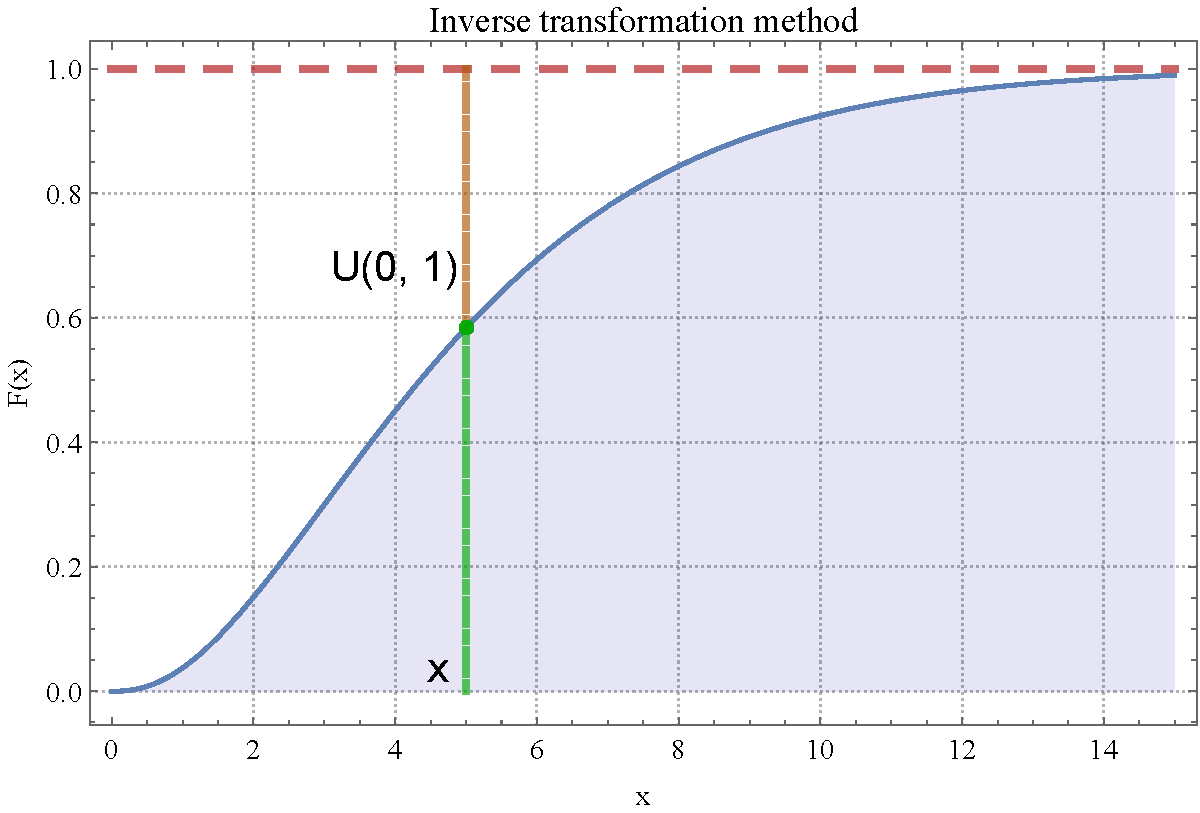
\includegraphics{monte_carlo/inverse_transformation_method.pdf}
	\caption[Inverse-transformation method.][6pt]{Generate non-uniform random number by using inverse-transformation method.}
	\label{fig:inverse_transformation_method}
\end{figure}

\subsection{Gaussian generator using central limit theorem}
\label{subsec:gaussian_generator}

$\to$ It works, but

\begin{enumerate}
	\item It is \mono{fucking} inefficient.
	\item It is truncated.
\end{enumerate}

\newthought{Exercise}: \nameref{exer:gaussian_random_number_generator}.

\subsection{Acceptance-rejection method (hit-or-miss method)}\index{acceptance-rejection}\index{hit-or-miss}
\label{subsec:acceptance_rejection}

Assume a PDF $f(x)$ defined in interval $[x_{1}, x_{2})$.

Assume we know $m = \max \left\{ f(x), x \in [x_{1}, x_{2}) \right\}$.

Then we can do the following:

\begin{enumerate}
	\item Generate a uniform number $x$ in $[x_{1}, x_{2})$.
	\item Generate a uniform number $r$ in $[0, m)$.
	\item If $f(x) > r$, we accept $x$, otherwise, we go back to 1. . (Figure~\ref{fig:acceptance_rejection})
	\item Populate a histogram with the accepted values. This will approximate the original $f(x)$ for large number of generated points.
\end{enumerate}

\begin{figure}
	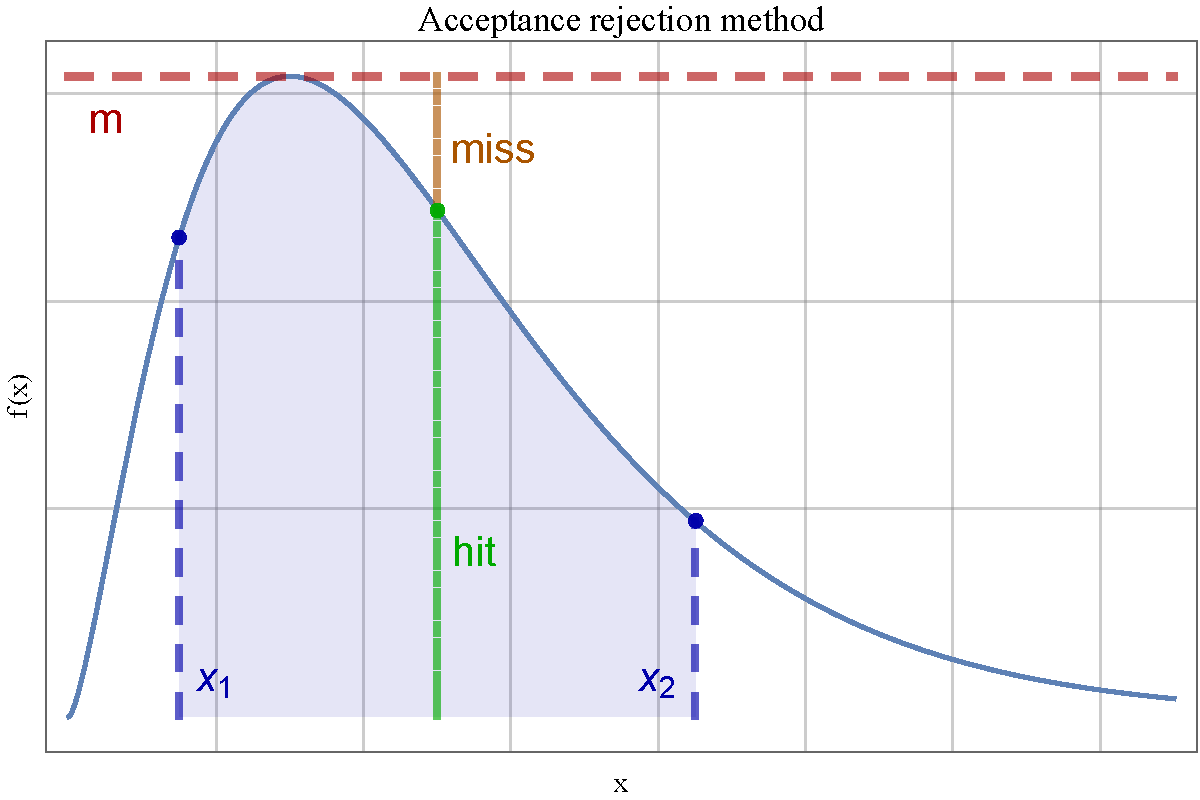
\includegraphics{monte_carlo/acceptance_rejection_method.pdf}
	\caption[Acceptance-rejection method.][6pt]{Generate non-uniform random number by using acceptance-rejection method.}
	\label{fig:acceptance_rejection}
\end{figure}

\subsection{Properties of acceptance-rejection method}\index{acceptance-rejection!property}
\label{subsec:prop_of_acceptance_rejection}

\begin{itemize}[$\to$]
	\item The method works well if we can compute $f(x)$ fast enough, but if $F(x)$ is computationally intensive.
	\item We only get a binned approximation of $f(x)$.
	\item The efficiency of the method is:
		$$
		\varepsilon = \frac{\int_{x_{1}}^{x_{2}}{f(x)} \,\mathrm{d}x}{(x_{2} - x_{1}) \cdot m}
		$$
		Therefore, it is inefficient if $f(x)$ is very peaked.
	\item It can be applied to multi-dimensional cases, but leads to the “curve of dimensionality”.
\end{itemize}

\newthought{Example}: \nameref{exer:acceptance_rejection}.

\subsection{Combination of random variables}
\label{subsec:combination_of_random_var}

For complicated cases, we can combine the inverse-transformation method and the acceptance-rejection method.

We can also use random number generator to produce binned PDFs of variables that are a combination of other variables.

This is for example the case of the ratio of two variables.

\newthought{Example}: \nameref{exer:change_of_var}.
